\begin{figure}[t]
  \centering
  \vspace{2mm}
  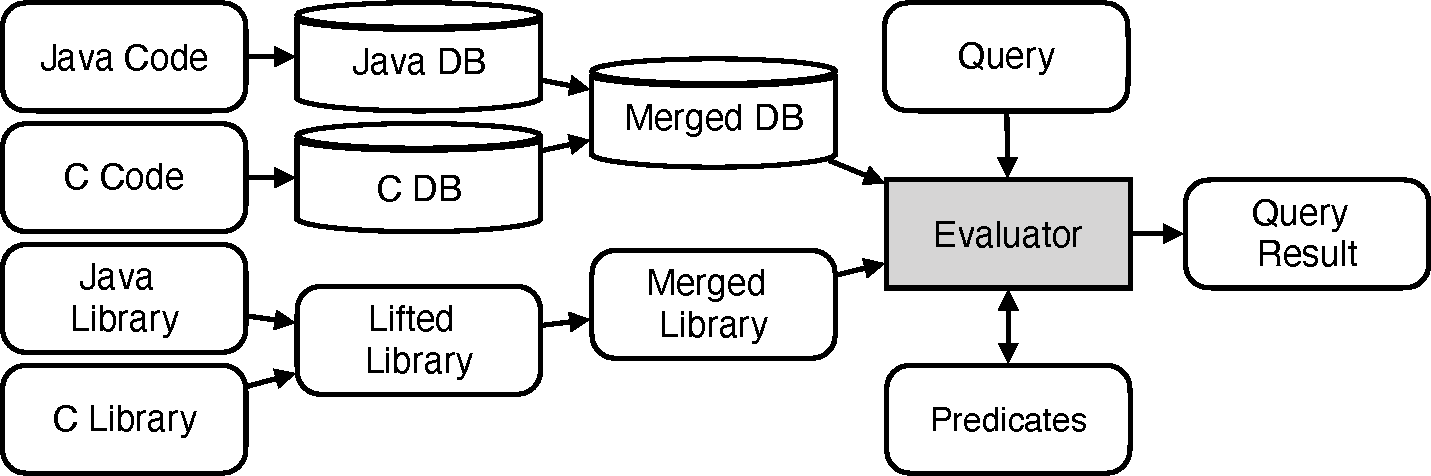
\includegraphics[width=0.47\textwidth]{img/codeql.pdf}
  \caption{Overall structure of MultiQL}
  \label{fig:codeql}
\end{figure}

%\section{Implementation}\label{sec:impl}
\section{MultiQL: Extension of CodeQL for multilingual program analysis}\label{sec:impl}
In this section, we present MultiQL, a prototype extension of
CodeQL~\cite{codeql} for multilingual program analysis.  MultiQL tracks
dataflows across language boundaries in two types of multilingual programs:
Java-C programs interperating via Java Native Interface(JNI)~\cite{jnispec} and
Python-c programs interoperating via Python Extension Module~\cite{pyext}.
Without loss of generality, we mainly explain our extension about the Java-C
program analysis throughout most of the section, since the only difference in
extensions between the Java-C program analysis and the Python-C program
analysis is to define language-interoperation rules.

%In this section, we present MultiQL, a prototype implementation of our
%approach of extending declarative static analysis for multilingual programs,
%in the case of dataflow analysis for JNI programs(Java-C)
%and extension module programs(Python-C) using CodeQL~\cite{codeql}.
%Dataflow analysis is an analysis to determine if a value that is created at
%certain program location, source, can flow into another certain program location, sink.
%Without loss of generality, we will mainly explain analysis of JNI program
%analysis throughout most of the section, since the difference between JNI programs and
%extension module programs is relevent only when defining
%language-interoperation rules.



\subsection{CodeQL}
%CodeQL is a static analysis engine that transforms source code programs into
%databases, and performs analysis by evaluating queries written in the
%declarative and object-oriented language called QL (Query Language).
%In QL, there are mainly two syntax for defining rules.
%They are defining ``predicates'' or ``classes.''
%The following QL code defines the predicate \codeql{isOneOrTwo}:

CodeQL is a declarative static analysis engine that transforms source code into
a database of facts and performs analyses by evaluating queries written in the
declarative and object-oriented language called QL (Query Language).  In QL,
one can define rules by defining ``predicates'' and ``classes.'' The following
QL code defines the predicate \codeql{isOneOrTwo}:

\begin{lstlisting}[style=codeql,xleftmargin=2.5em]
predicate isOneOrTwo(int n) {
  n = 1
  or
  n = 2
}
\end{lstlisting}

\noindent
and the following definition defines the class \codeql{OneOrTwo}:

\begin{lstlisting}[style=codeql,xleftmargin=2.5em]
class OneOrTwo extends int {
  OneOrTwo() { // characteristic predicate
    this = 1
    or
    this = 2
  }
}
\end{lstlisting}

\noindent
A class defines a set of elements that satisfy the predicate called
``characteristic predicate.'' For more information about QL, one can refer to
\citet{ql2016}'s paper or the official document~\cite{codeql}.

%Figure~\ref{fig:codeql} presents the overall structure of MultiQL for JNI programs.
%First, it generates databases for both languages, C\footnote{
%Even though MultiQL analyzes JNI programs written in Java and both C and
%C++, this paper refers to C only fore presentation brevity.} and
%Java, and merges them to one database.  This corresponds
%to the step of extracting syntactic datafacts from source code programs.
%Then, we merge the common datafacts and rules in both languages,
%which are parts of their libraries that CodeQL provides, into one merged library.
%Finally, using the merged database and merged library, a user can write a query to
%perform a client-analysis, and evaluate it to produce its analysis result.

Figure~\ref{fig:codeql} presents the overall structure of MultiQL for JNI
programs.  First, it generates databases for both languages, C\footnote{ Even
though MultiQL analyzes JNI programs written in Java and both C and C++, this
paper refers to C only for presentation brevity.} and Java, and merges them to
one database.  This corresponds to the step of extracting syntactic initial
facts from source code.  Then, we merge the common facts and rules in both
languages, which are parts of their libraries that CodeQL provides, into one
merged library.  Finally, using the merged database and merged library, a user
can write a query to perform a client-analysis, and evaluate it to produce its
analysis result.

\subsection{Creating Databases}
For compiled languages such as C and Java, CodeQL generates their database by
compiling source programs.  When a compiler compiles a program, CodeQL monitors
the compiler to extract necessary information and creates a database with the
extracted information. For script languages like Python, CodeQL uses its own
extractor to directly extract necessary information from source code.
CodeQL creates a database for a single language in two steps:
1) it stores the extracted information in a trap
file, a human readable file format, and 2) it finalizes trap files
into databases in the binary format. For example, the
following demonstrates a sample trap file:

\begin{lstlisting}[style=java,numbers=none]
#10001=@"class;myClass.MyClass"  ...
#10002=@"type;int"
primitives(#10002,"int")  ...
#10003=@"callable;{#10001}.myMethod({#10002}){#10002}"  ...
#10004=@"params;{#10003};0"
params(#10004,#10002,0,#10003,#10004)
paramName(#10004,"myParam")
\end{lstlisting}

\noindent
which describes the parameter information about \javacode{myMethod}.
\javacode{primitives(...)}, \javacode{params(...)}, and
\javacode{paramName(...)} are facts stored in tables in the database.  The
database manages tables based on fact types. For example, it stores the kind of
facts \javacode{primitives(...)} in a table named \javacode{@primitives}, and
\javacode{params(...)} in a different table named \javacode{@params}.

%Here, each line of \javacode{primitives(...)},
%\javacode{params(...)}, and
%\javacode{paramName(...)}
%corresponds to one fact, which will be
%finally stored in each table of database.

\begin{figure}[t]
  \centering
  \vspace{2mm}
  \begin{subfigure}[t]{0.5\textwidth}
\begin{lstlisting}[style=codeql,xleftmargin=2.5em]
class Node extends TNode { ... }
predicate simpleLocalFlowStep(Node from, Node to) {
  exprToExprStep_nocfg( // Expr -> Expr
    from.asExpr(),
    to.asExpr()
  )
  or ...  // Assignment -> LValue post-update node
}
\end{lstlisting}
    \vspace*{-.5em}
    \caption{c/dataflow/internal/DataFlowUtil.qll}
  \end{subfigure}
  \begin{subfigure}[t]{0.5\textwidth}
\begin{lstlisting}[style=codeql,xleftmargin=2.5em]
class Node extends TNode { ... }
predicate simpleLocalFlowStep(Node node1, Node node2) {
  // Variable flow steps through
  // adjacent def-use and use-use pairs.
  exists(SsaExplicitUpdate upd |
    upd.getDefiningExpr().(VariableAssign).getSource()
      = node1.asExpr() or
    upd.getDefiningExpr().(AssignOp) = node1.asExpr()
  |
    node2.asExpr() = upd.getAFirstUse()
  )
  or ...  // Flow through this
}
\end{lstlisting}
    \vspace*{-.5em}
    \caption{java/dataflow/internal/DataFlowUtil.qll}
  \end{subfigure}
  \vspace*{-.5em}
  \caption{QL libraries for C and Java}
  \label{fig:qll}
\end{figure}

To create a single merged database for both C and Java, MultiQL maintains a
separate trap file for each language and then merges them.  
Note that both trap files may have tables with the same name.  
To avoid name conflicts in a merged database, we add a language-specific prefix
to each table.  
For example, if both trap files have tables named \codeql{@params}, we rename
the table from C as \codeql{@c\_params}, and the table from Java as
\codeql{@java\_params}.
After renaming such tables, we can safely finalize the trap files into
databases on which queries can be evaluated.

%To create a single database for both C and Java, MultiQL maintains
%a separate trap file for each language and then merges them.
%Note that both trap files may have tables with the same name.
%To avoid name conflicts in a merged database, we add a
%language-specific prefix to each table.
%For example, if both trap files have tables named \codeql{@params},
%we rename the table from C as \codeql{@c\_params},
%and the table from Java as \codeql{@java\_params"}.
%After renaming such tables, we can safely finalize the trap files into
%databases on which queries can be evaluated.

\subsection{Lifting Libraries}

CodeQL provides various libraries for C and Java, including
pre-defined predicates and classes for users to implement their own analyses.
A dataflow analysis library is such a library, which supports both C and Java.
For example, Figure~\ref{fig:qll} shows sample QL libraries for C and Java,
which uses the same class name \ccode{Node} and the same predicate
name \ccode{simpleLocalFlowStep}.
However, even with the same name, the class \ccode{Node} in C and the
class \javacode{Node} in Java are different classes, which are incompatible.
The same applies to the predicate \ccode{simpleLocalFlowStep}.
In other words, we can not use the class \ccode{Node} in C as an
argument of the predicate \javacode{simpleLocalFlowStep} in Java or vice versa.

To make classes and predicates in C and Java become compatible,
we lift each library to the common level.
First, we encapsulate each of the original dataflows in a CodeQL
module named C and JAVA so that we can distinguish the original
classes and predicates by lifted ones.
We can lift a class by first defining a sum type, denoting that
the lifted class comes either from C or Java, and then making the
lifted class be of that type.  We also implement two member predicates
that can cast the lifted class into the C or Java class:
\begin{lstlisting}[style=codeql,xleftmargin=2.5em]
private newtype TNode =
  TJavaNode(JAVA::Node n)
  or
  TCNode(C::Node n)
class Node extends TNode {
  JAVA::Node asJava() {
    this = TJavaNode(result)
  }
  C::Node asC() {
    this = TCNode(result)
  }
  ...
}
\end{lstlisting}
Similarly, we can lift a predicate by combining two original predicates with
the \codeql{or} connective. For each original predicate, we cast down
each of the arguments and return values to the class of its corresponding language:
\begin{lstlisting}[style=codeql,xleftmargin=2.5em]
predicate simpleLocalFlowStep(Node node1, Node node2) {
  JAVA::simpleLocalFlowStep(
    node1.asJava(), node2.asJava()
  )
  or
  C::simpleLocalFlowStep(
    node1.asC(), node2.asC()
  )
}
\end{lstlisting}
After lifting, lifted predicates show the equivalent behaviors as the
original ones if all the arguments are from the same language.

We fully automate the lifting process with the aid of QL compiler error
messages. When compiling a query with the merged database, the QL compiler
reports error messages containing required classes and predicates, and a
signature of each required predicate. Using the information, we synthesize
lifted classes and predicates without manually efforts.

%The process of lifting could be effectively automated with the aid of
%QL's compile message. First, try to compile a query without actually
%importing the library, then the QL compiler will give error message
%that contains all the iinformation about required yet missing predicates and classes,
%such as name, arity or signature of each predicate. Using this information,
%the lifted predicates and classes can be automatically synthesized, without
%manually searching for what are the required ones.

\subsection{Merging Libraries: Java-C}\label{sec:merging}
After lifting libraries for different languages, we extend predicates to
reflect the interoperation semantics between multiple languages.  
For the Java-C program analysis, we identified various interactions from Java
to C and from C to Java via JNI, and extended predicates to model their
behaviors.

%After lifting libraries for different languages, we extend predicates to
%reflect the interoperation semantics between multiple languages.
%For analyzer for JNI programs, We identified various interactions from Java to C and from C to Java
%and extended predicates to model their behaviors.

For example, the following shows how we extend the predicate
named \codeql{viableCallable}:
\begin{lstlisting}[style=codeql,xleftmargin=2.5em]
DataFlowCallable viableCallable(DataFlowCall c) {
  result.asJava() = JAVA::viableCallable(c.asJava())
  or
  result.asC() = C::viableCallable(c.asC())
  or
  result.asC() = viableCallableJ2C(c.asJava())
  or
  result.asJava() = viableCallableC2J(c.asC())
}
\end{lstlisting}
%This predicate finds the call edge from the call expression to its
%target, and is required for finding data flows through the fnction arguments and returns.

\noindent
The predicate \codeql{viableCallable} finds call edges from call expressions to
their targets. 
Lines 2 and 4 show the results of lifting, and they take advantage of the
original predicates from the dataflow libraries.  
They handle intra-language call edges from Java to Java and from C to C.
Lines 6 and 8 show the results of merging libraries, and they are
for inter-language call edges.  The predicate \codeql{viableCallableJ2C} finds call edges
from Java to C, and the predicate \codeql{viableCallableC2J} finds call edges from
C to Java. Because these two call edges have different characteristics, we
implemented them differently.

%\medskip
\textbf{Java to C.} In Java-C programs, one can make interactions from Java to
C by calling native functions in C from Java code. 
The target of such a function call is determined in a static manner.
The target function should follow the JNI naming convention, which is adding
\codeql{Java\_} as prefix, followed by a fully qualified name of its class and
the additional \codeql{\_}, to the method name.
For example, the target function name for a function call of \codeql{cfunction}
would be \codeql{Java\_fully\_qualified\_class\_name\_cfunction}.
With this convention, we can define \codeql{viableCallableJ2C} so that
\codeql{f = viablaCallableJ2C(call)} holds when \codeql{f.toString() = "Java\_"
+ call.getTarget().className() + "\_" +} \\
\codeql{call.getTarget().getName()} holds.


\medskip
\textbf{C to Java.} The interaction from C to Java is more complex and
requires more careful implementation than the interaction from Java to C.
The primary difference is that a method call from C to Java requires knowing
the runtime values of variables, which may not be always possible.
First, C code calls the interface function \ccode{GetMethodID(name, sig)}
to get the ``method ID'' of the method whose name matches the first argument
and the type signature matches the second argument passed to this function.
This method ID is stored at a variable, say \ccode{mid}, and
an actual method call is invoked by another
interface function, \ccode{Call<type>Method(obj, mid, args...)}. Calling this interface 
function corresponds to calling the method that \ccode{mid} indicates
with \ccode{obj} as ``this object'' and \ccode{args} as the arguments.

To correctly handle this method call, we should be able to answer these
questions: ``When we call \ccode{GetMethodID},
what are the string values of \ccode{name} and \ccode{sig}?'' and
``When we call \ccode{Call<type>Method}, what is the method ID value of \ccode{mid}?''
Answering these questions requires dataflow analysis;
to soundly answer to them, inter-language dataflow analysis is necessary.
However, in practice, intra-language dataflow analysis is enough in most cases.
Therefore, we implemented two ``intra-flow'' analysis modules for C,
which find 1) dataflows from string literals to the arguments of interface functions,
and 2) dataflows from interface function call results to the arguments of interface functions.
Using these modules, we can implement the
predicate \codeql{viableCallableC2J} by adding a call edge from a \ccode{Call<type>Method}
call to the method \ccode{m}, if there is a flow to \ccode{mid} from a
call to \ccode{GetMethodID}, and string values that flow into the
arguments \ccode{name} and \ccode{sig} of \ccode{GetMethodID} that
correspond to the name and the type signature of the method \ccode{m}.

In addition to the predicate \codeql{viableCallable},
we extended more predicates to consider other JNI interface functions such as
\ccode{findClass} and \ccode{GetFieldID}.
Most of such extended predicates are specialized \codeql{step} predicates.
We extended them in a similar way to the calls from C to Java described above.

\subsection{Merging Libraries: Python-C}\label{sec:merging2}
%The extension module programs requires its own modelling for its own interoperation
%semantics to be analyzed.
%The following is the extension of the predicate \codeql{viableCallable}
%for extension module programs:

To analyze Python-C programs, we extended predicates to model the
interoperation semantics of Python Extension Module.
The following shows the \codeql{viableCallable} predicate we extened for the
Python-C program analysis: 

\begin{lstlisting}[style=codeql,xleftmargin=2.5em]
DataFlowCallable viableCallable(DataFlowCall c) {
  result.asPython() = PYTHON::viableCallable(c.asPython())
  or
  result.asC() = C::viableCallable(c.asC())
  or
  result.asC() = viableCallableP2C(c.asPython())
  or
  result.asPython() = viableCallableC2P(c.asC())
}
\end{lstlisting}

\noindent
The only different parts from the Java-C program analysis are the predicates
\codeql{viableCallableP2C} and \codeql{viableCallableC2P}, which we describe in
next paragraphs.

%Again, line 2 and line 4 are direct outcomes of the process of lifting,
%and all we have to newly define is the language-interoperation predicates,
%\codeql{viableCallableP2C} and \codeql{viableCallableC2P}. 

\textbf{Python to C.} Similar to the interactions from Java to C, one can make
interactions from Python to C by importing and calling functions exported from
C. Python Extension Module provides a pre-defined C struct \ccode{PyMethodDef} to
export a C function to Python: 
%Similar to JNI programs,
%in python program with 
%extension modules, one can make interactions from
%Python to C by importing and calling C functions that are exported via
%extension modules. There is a C structure "PyMethodDef"
%that stores the information about the c function that is exported. If we define
%the structure

\begin{lstlisting}[style=mcpp]
struct PyMethodDef methods[] = {
  {
    .ml_name = "cfunction",
    .ml_meth = cfunction_imp,
    ...
  },
  ...
}
\end{lstlisting}

\noindent
The member field \ccode{ml_name} has a visible name of a C function to Python,
and the member field \ccode{ml_meth} has the actual name of the C function.
Thus, the \ccode{cfunction_impl} function defined in C code is invoked when
importing and calling \ccode{cfunction} in Python code.
\inred{To model the behavior, we can define \codeql{viableCallableP2C} so that
\codeql{f = viablaCallableP2C(call)} holds when \codeql{f = def.getFunc()} and
\codeql{call.getTarget().toString() = def.getName()} holds. TODO: what is the
{\tt def}?}

In addition, we define rules that connects dataflows from arguments of
Python-to-C function calls to a parameter of the target C function. 
Different from the Java-to-C function call semantics, Python Extension Module
packs arguments in a Python tuple object and propagates the object to the sole
parameter of the target C function. 
Then, the target C function unpack the tuple object into individual Python
objects by calling the \ccode{PyArg_ParseTuple} API. 
\inred{
Then the
writter of c function should manually call API function,
\ccode{PyArg\_ParseTuple} to unpack this tuple to get each individual
arguments. This behavior is modelled by creating virtual argument node which is
a virtual Python tuple object, and create the store step from the real argument
to the virtual argument.  By doing so. the real argument will flow to the real
use site of in three steps: 1) store step from the argument to virtual
argument, 2) function-in step from virtual argument to the parameter of target
C function, and 3) read step from the parameter to its tuple-read API fuction.
The similar thing happens when there is a call from C to Python. The actual
argument of C API function is a tuple object, but this tuple is implicitly
unpacked and each element is assigned to each parameter of Python method.
Again, the solution is to create virtual parameter in Python, and create the
read step from the virtual tuple parameter to actual parameters.
}


%then the Python code can import cfunction and the call expression cfunction()
%will resolve to the actual function cfunction\_impl defined in C code. To model
%this behavior, we can define \codeql{viableCallableP2C} so that \codeql{f =
%viablaCallableP2C(call)} holds when \codeql{f = def.getFunc()} and
%\codeql{call.getTarget().toString() = def.getName()} holds.

\medskip
%\textbf{C to Python.} The interaction from C to Python also requires
%the runtime values of variables, which makes the analysis a bit complex. 
%C code calls the interface function \ccode{PyObject\_CallObject(func, args)}
%where func is the python function object, and the args is the python tuple
%object. Finding call target of this API function call simply reduces to answering the
%question: ``what is the value of \ccode{func}?'' Again, we define
%``intra-flows'' for both Python and C to answer this question efficiently: 1) dataflows from 
%python function any to arguments in Python and 2) dataflow from any parameters to the first argument of
%\ccode{PyObject\_CallObject} in C. Then, the value that \ccode{func} may have
%is found via three big steps: finding flow from Python function to an argument, from the argument to
%a c parameter, and from the parameter to the variable \ccode{func}.

\textbf{C to Python.} The interaction from C to Python requires the runtime
values of variables, similar to the interaction from C to Java. 
To invoke Python functions in C, C code calls the interface function
\ccode{PyObject_CallObject(func, args)}, where the \ccode{func} is a Python
function object, and the \ccode{args} is a Python tuple object. 
Because C code can get Python objects only propagated from Python code as
function arguments of the Python-to-C interoperation, we define two
``intra-flows'' analyses to identify Python objects assigned to \ccode{func}:
1) dataflows from Python to C function arguments, and 2) dataflows from C
function parameters to the first argument of \ccode{PyObject_CallObject}. 
\inred{Then, the value that \ccode{func} may have
is found via three big steps: finding flow from Python function to an argument, from the argument to
a c parameter, and from the parameter to the variable \ccode{func}.}


%\textbf{Args and Params.} After finding the call target of the given call
%expression, Then we have to connect the dataflow from the arguments to
%aprameters.  This is tirivial for JNI programs, but in case of extension module
%programs, it requires a bit of effort. When you call a c function from the
%Python code with arguments, then all the arguments are implicitly packed in a
%tuple, and that tuple is passed to c function as a single argument. Then the
%writter of c function should manually call API function,
%\ccode{PyArg\_ParseTuple} to unpack this tuple to get each individual
%arguments. This behavior is modelled by creating virtual argument node which is
%a virtual Python tuple object, and create the store step from the real argument
%to the virtual argument.  By doing so. the real argument will flow to the real
%use site of in three steps: 1) store step from the argument to virtual
%argument, 2) function-in step from virtual argument to the parameter of target
%C function, and 3) read step from the parameter to its tuple-read API fuction.
%The similar thing happens when there is a call from C to Python. The actual
%argument of C API function is a tuple object, but this tuple is implicitly
%unpacked and each element is assigned to each parameter of Python method.
%Again, the solution is to create virtual parameter in Python, and create the
%read step from the virtual tuple parameter to actual parameters.
